% standard
\documentclass[a4paper,12pt]{article}
\usepackage[utf8]{inputenc}
\usepackage[ngerman]{babel}

% geometry
\usepackage{geometry}
\geometry{ headsep=20pt,
headheight=20pt,
left=21mm,
top=15mm,
right=21mm,
bottom=15mm,
footskip=20pt,
includeheadfoot}

% header and footer
\usepackage{datetime}
\newdateformat{dmy}{%
\THEDAY.~\monthname[\THEMONTH] \THEYEAR}
\usepackage{fancyhdr}
\pagestyle{fancy}
\lhead{Noah Vogt \& Simon Hammer}
\chead{}
\rhead{\dmy\today}
\lfoot{}
\cfoot{Gymnasium Kirschgarten}
\rfoot{Seite \thepage}
\renewcommand{\footrulewidth}{.4pt}

%for the circuit
\usepackage[siunitx, european]{circuitikz}

% fix figure positioning
\usepackage{float}

% larger inner table margin
\renewcommand{\arraystretch}{1.4}

% no paragraph indent
\setlength{\parindent}{0em}

% graphics package
\usepackage{graphicx}

\usepackage{multicol}

% use sans serif font
\usepackage{tgheros}
\usepackage{mathptmx}

% don't even ask what this is for, I have no idea (noah)
\usepackage{bm} %italic \bm{\mathit{•}}
\usepackage[hang]{footmisc}
\usepackage{siunitx}
\usepackage[font={small,it}]{caption}
\sisetup{locale = DE, per-mode = fraction, separate-uncertainty,   exponent-to-prefix, prefixes-as-symbols = false, scientific-notation=false
}
\newcommand{\ns}[4]{(\num[scientific-notation=false]{#1}\pm\num[scientific-notation=false]{#2})\cdot\num[]{e#3}\si{#4}}

% show isbn in bibliography
\usepackage{natbib}

\usepackage{amsmath}

\begin{document}

\begin{titlepage}

\vspace*{1cm}
	\centering
	
	{\scshape\Large Protokolle Praktikum Physik 3cg \par}
	\vspace{0.5cm}
	{\huge\bfseries Die experimentelle Prüfung der Kirchhoff'schen Gesetze\par}
	\vspace{0.5cm}
	{\Large Noah Vogt \& Simon Hammer\par}
	\vspace{17cm}

	{\large Durchgeführt am 26.Januar 2021\par}
	
\end{titlepage}

\tableofcontents
\pagebreak

\section{Versuchsziel}
Die Kirchhoff'sche Gesetze sollen mittels eines Experiments überprüft werden. Dazu wurde ein Schaltkreis vorgegeben, der auf einem Steckbrett nachkonstruiert werden sollte. Mit einer praktischen Messung von Spannung und Stromstärke an spezifischen Stellen der Schaltung und getrennter theoretischer Berechnung der Schaltung mithilfe der Kirchhoff'schen Gesetze sollten die oben erwähnten Gesetzmässigkeiten nach ihrer Richtigkeit überprüft werden. Es wird erwartet, dass die theoretischen Werte dabei über den praktischen Werten liegen werden.\\

Wenn nämlich die Rechnung und gemessenen Werte - im Rahmen einem gewissen zu erwartenden Fehlerbereich - übereinstimmen, sind die Gesetze experimentell bestätigt.
\section{Physikalischer Hintergrund}

\subsection{Kirchhoffischen Gesetze}
\subsubsection{Maschenregel}

Wird ein geschlossener Teilstromkreis ("Masche") betrachtet so gilt, dass die Summe der 
Teilspannungen der der Totalspannung entspricht. Liegt an der Masche kein Spannungsquelle an so
gilt:

\[\sum_{k = 1}^{n} I_k = 0 \]
%\[ \sum_{n=0}^N


\subsubsection{Knotenregel}

Die Summe der eingehenden Ströme ist gleich der Summe der ausgehend Ströme in jedem 
Verzweigungspunkt ("Knoten"):

\[\sum I_{ein} = \sum I_{aus}\]


\subsection{Serieschaltung}

\begin{figure}[H]

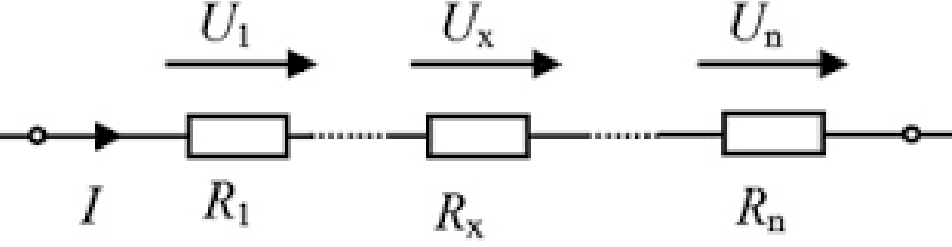
\includegraphics[width=.4\textwidth]{media/SerieschaltFert.png}

Die Knotenregel sagt aus, dass der selbe Strom $I_0$ durch alle Widerstände $R_i$ fliesst. Durch
die Maschenregel ergibt sich dann:

\[U_0 = \sum_{k=1}^{n} R_k I_0 ,\ I_0 = \frac{U_0}{\sum_{k=1}^{n} R_k }\] 

Die Spannung teilt sich somit direkt proportional auf die einzelnen Widerstände auf.

\end{figure}

\newpage

\subsection{Parallelschaltung}

\begin{figure}[H]

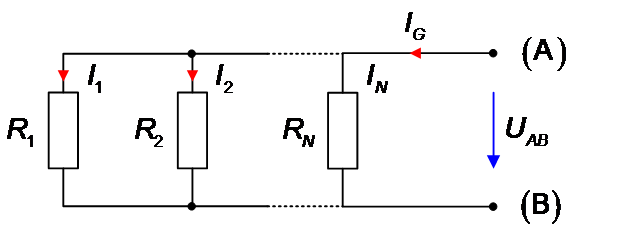
\includegraphics[width=.4\textwidth]{media/ParallelschaltungFert.png}

\end{figure}

Nach der Maschenregel liegt über allen Widerständen die gleiche Spannung $U_0$ und nach der 
Knotenregel beträgt die Summe der Teilströme den Gesamtstrom $I_0$:

\[ I_0 = \sum_{k=1}^{n} I_k \]

und 

\[ U_0 = R_1 I_1 = R_2 I_2 = ...R_n I_n \]

Der Strom wird also indirekt Proportional zu den Widerständen aufgeteilt. \\
Nach Auflösen der zweiten Gleichung nach $I_j$ mit $1 \leq j \leq n$ und einsetzen in die erste
ergibt sich:

\[ I_0 = \frac{U_0}{R_1} + \frac{U_0}{R_2} + ... + \frac{U_0}{R_n} = U_0 \sum_{n=1}^k \frac{1}{R_n} \]



\subsection{Ersatzwiderstand}

Die Gesamtstromstärke $I_0$, ist die Stromstärke, welche vor dem ersten Knoten herscht. \\
Die Gesamtspannung $U_0$, ist die Spannung, welche an das Stromnetz angelegt wird. \\
Wird das ganze Widerstandsnetz mit einem Widerstand ersetzt, so heisst dieser Ersatzwiderstand. 

\[ R_E = \frac{U_0}{I_0} \]

Der Ersatzwiderstand verändert \textit{nicht} die Gesamtstromstärke. 

\section{Versuchsaufbau}
%\begin{figure}[H]

%\centering
%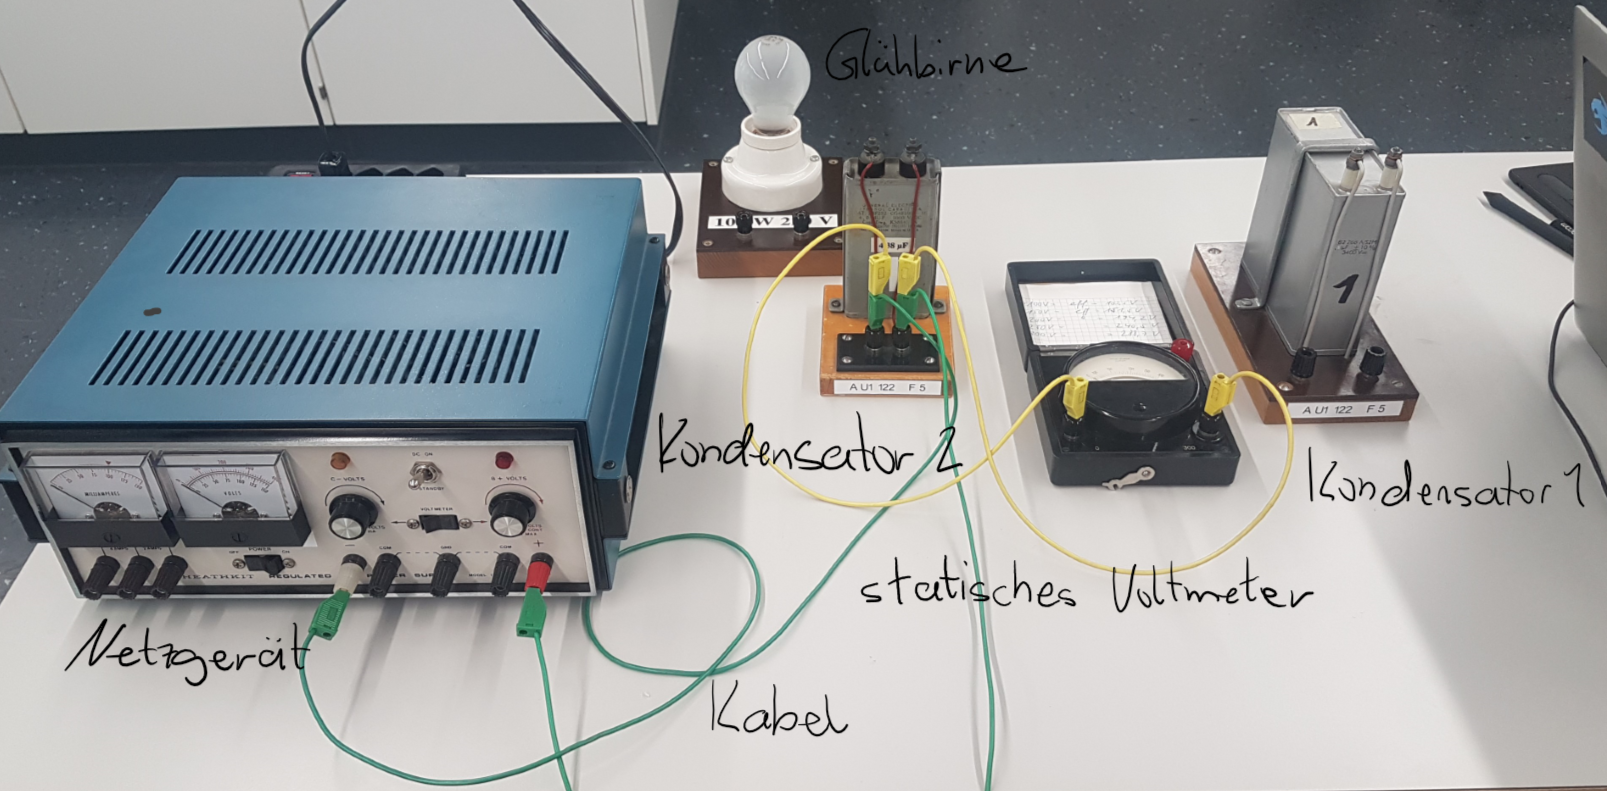
\includegraphics[width=.8\textwidth]{media/bennenung.png}
\begin{figure}[H]
\centering
\rotatebox[origin=c]{90}{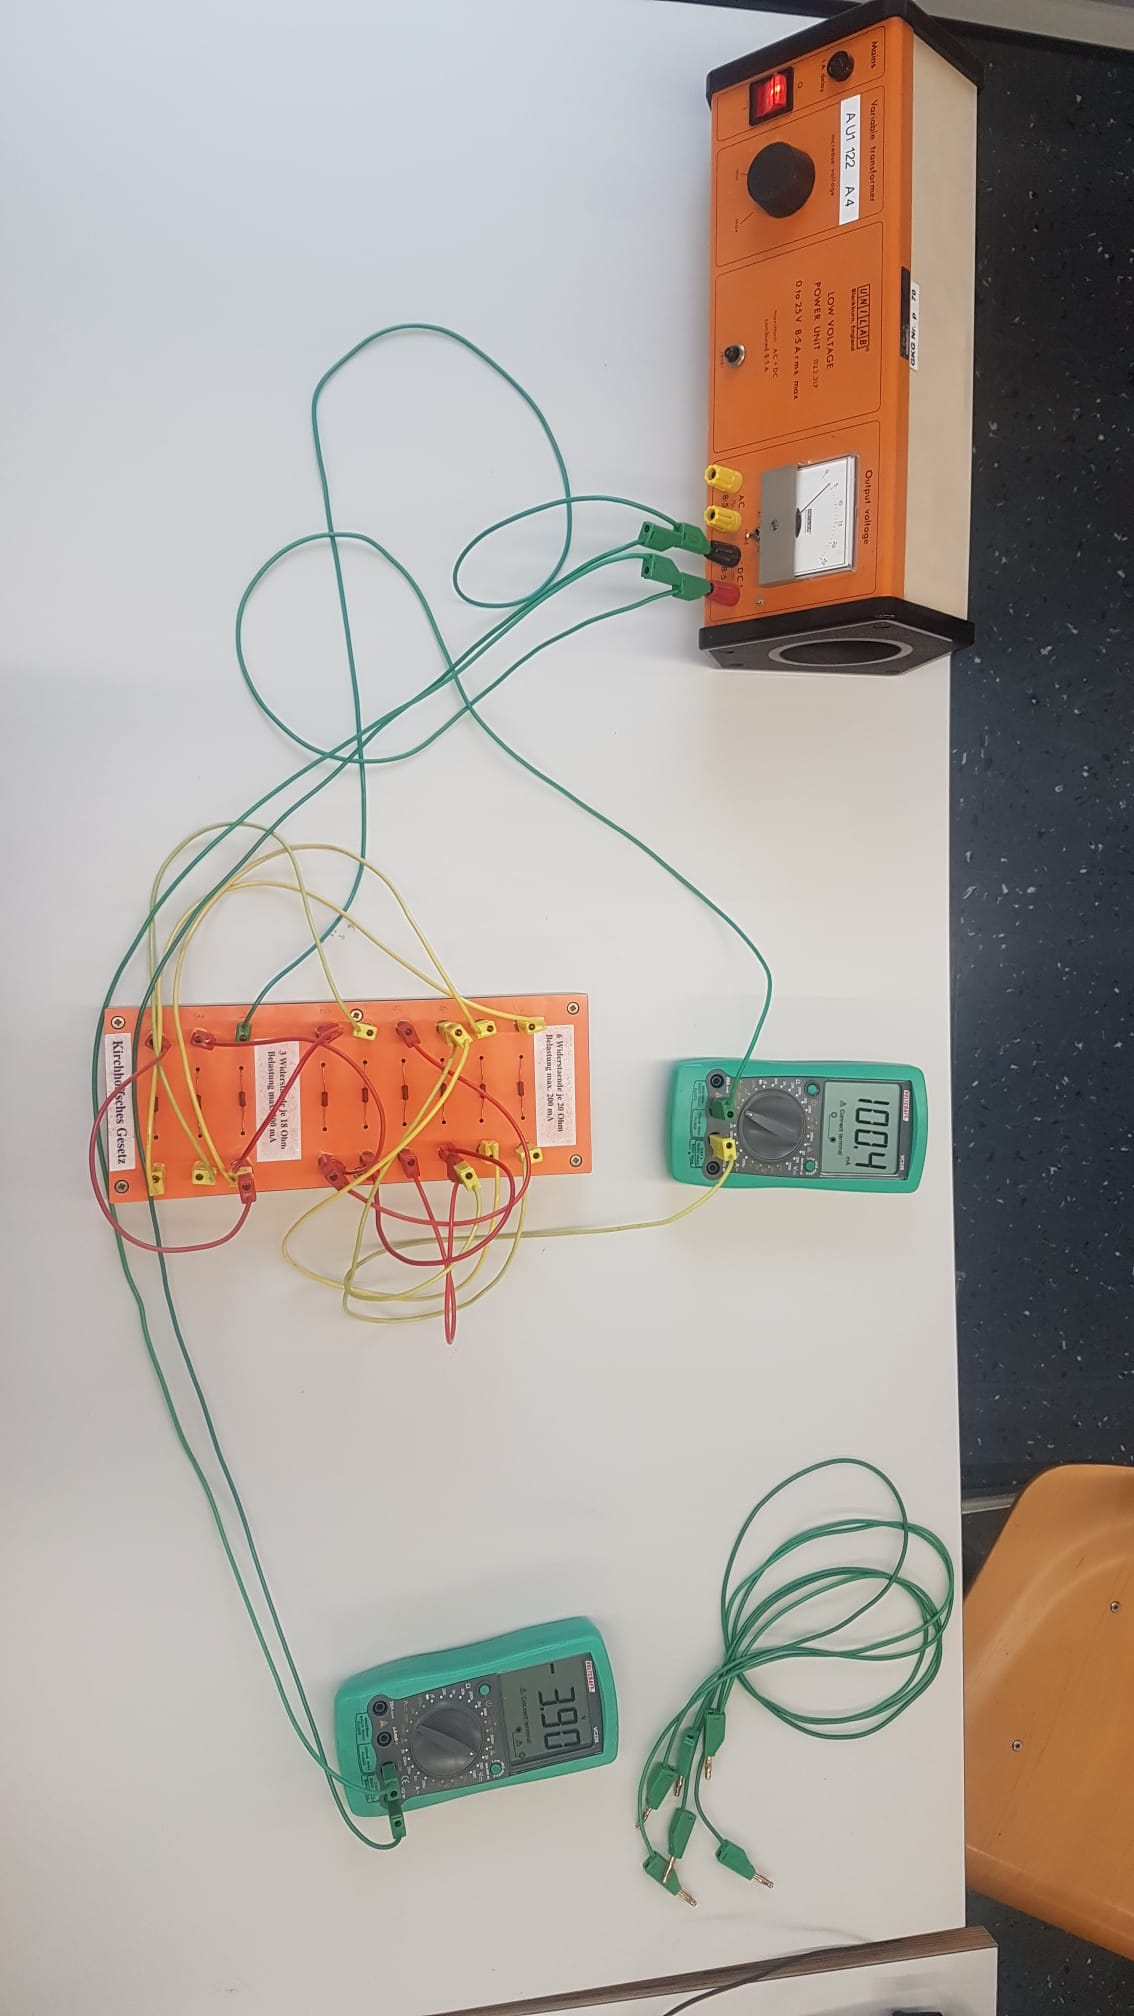
\includegraphics[width=.5\textwidth]{media/ExpSchaltQuerAll.jpeg}}
\end{figure}


\begin{center}
\begin{circuitikz}[scale = 2.2]

    %circuit
    \draw (0,0) 
        to[isource, l=$I_0$, i=$I_0$] (4,0) 
        to [R=$R_1$ (\SI{18}{\ohm}), -*] (4,2)
        to [R=$R_2$ (\SI{20}{\ohm}), -*] (3,2)
        to [short]     (3,1.5)
        to [R=$R_3$ (\SI{18}{\ohm})]     (2,1.5)
        to [R=$R_4$ (\SI{20}{\ohm})]     (1,1.5)
        to [short, -*] (1,2)
        to [short, -*] (0,2)        
        to[ammeter, l=$A$] (0,0) --  (0,0);

    \draw (1,2)
        to [short] (1,2.5)
        to [R=$R_5 $(\SI{20}{\ohm})] (3,2.5) 
        to [short] (3,2);
    
    \draw (0,2)
        to [R=$R_6$ (\SI{20}{\ohm})]     (0,4)
        to [short, -*] (1,4)
        to [short]     (1,3.5)
        to [R=$R_7$ (\SI{20}{\ohm})]     (3,3.5)
        to [short, -*] (3,4)
        to [short]     (4,4)
        to [short]     (4,2);

    \draw (1,4)
        to [short]      (1,4.5)
        to [R=$R_9$ (\SI{20}{\ohm})]      (2,4.5)
        to [R=$R_8$ (\SI{18}{\ohm})]      (3,4.5)
        to [short]      (3,4);

    %arrows
    \draw (3.85,2)node[flowarrow,color = red, rotate = 180, label = \color{black}$I_1$]{};
    \draw (3,2.13)node[flowarrow,color = red, rotate = 90, label = left: \color{black}$I_3$]{};
    \draw (3,1.8)node[flowarrow,color = red, rotate = -90, label = left: \color{black}$I_4$]{};
    \draw (0.85,2)node[flowarrow,color = red, rotate = 180, label = \color{black}$I_1$]{};
    \draw (4,2.13)node[flowarrow,color = red, rotate = 90, label = right: \color{black}$I_2$]{};
    \draw (3,4.13)node[flowarrow,color = red, rotate = 90, label = left: \color{black}$I_5$]{};
    \draw (3,3.8)node[flowarrow,color = red, rotate = -90, label = left: \color{black}$I_6$]{};
    \draw (0.85,4)node[flowarrow,color = red, rotate = 180, label = \color{black}$I_2$]{};
    \draw (0,1.8)node[flowarrow,color = red, rotate = -90, label = left: \color{black}$I_0$]{};

\end{circuitikz}
\end{center}

\section{Versuchsdurchführung}

\begin{table}[H]
    \centering
    \begin{tabular}{|c|c|}
        \hline
         & \textbf{gemessene Spannung U [V]}\\
        \hline
        $U_{Netz}$ & $3.90\pm 0.005$\\
        \hline
        $U_1$ & $1.78\pm 0.005$\\
        \hline
        $U_2$ & $1.00\pm 0.005$\\
        \hline
        $U_3$ & $0.31\pm 0.005$\\
        \hline
        $U_4$ & $0.34\pm 0.005$\\
        \hline
        $U_5$ & $0.65\pm 0.005$\\
        \hline
        $U_6$ & $1.02\pm 0.005$\\
        \hline
        $U_7$ & $0.63\pm 0.005$\\
        \hline
        $U_8$ & $0.30\pm 0.005$\\
        \hline
        $U_9$ & $0.33\pm 0.005$\\
        \hline
    \end{tabular}
\end{table}

Zuerst wurde nach Vorgabe das ganze Steckbrett mit den integrierten Widerständen verkabelt und das Ampèremeter angeschlossen. Entsprechend den herrschenden Widerständen und erwarteten maximalen Stromstärken und Spannungen mussten die Einstellungen an Volt- und Ampèremeter angepasst werden. Nach genauem Nachkontrollieren, ob das Steckbrett wirklich korrekt aufgebaut worden ist, wurde schliesslich das Netzgerät an die Schaltung angeschlossen. \\

Dann wurde die Spannung am Netzgerät erhöht, sodass die Funktionalität der Widerstände sich zeigen konnte. Das Voltmeter wurde für die Messungen einzeln zu jedem Widerstand parallelgeschalten und der angezeigte Wert wurde abgelesen. Mit einer Achtung darauf, ob eines der Kabel, Messgeräte oder Widerstände durchbrennt, wurde das Netzgerät noch wenige Minuten angelassen. Es wurde aber auch darauf geachtet, dass sich kein Wasser in der Nähe des Versuchesaufbaues befand und um den Fall eines durchbrennenden Widerstands vorbeugend zu minimieren.\\

Nach erfolgreichem Abschluss der Messung wurde das Netzgerät wieder abgeschaltet, vom Netz getrennt und alle sonstigen am Steckbrett angeschlossenen Gerätschaften wieder entfernt und versorgt.

\newpage

\section{Versuchsauswertung}

\subsection{Ersatzwiderstände berechnen}

Um die obere Masche mit den Widerständen $R_7$, $R_8$ und $R_9$ (siehe Schaltkreis in 3.) zu vereinfachen, beginnen zuerst mit der Vereinfachung der Serieschaltung:

$$R_{8,9} = R_9 + R_8 = 20\;\Omega + 18 \;\Omega = 38 \;\Omega$$

Dann folgt die Parallelschaltung:

$$R_{7,8,9} = \frac{R_{8,9} \cdot R_7}{R_{8,9} + R_7} = \frac{38 \;\Omega \cdot 20\; \Omega}{38\; \Omega + 20\; \Omega} = \frac{380}{29}\Omega$$\\

Analog dazu lässt sich der obere Rechenweg auch anwenden auf die untere Masche mit $R_3$, $R_4$ und $R_5$:  

$$R_{3,4} = R_4 + R_3 = 20 \;\Omega + 18 \;\Omega = 38 \;\Omega$$

$$R_{3,4,5} = \frac{R_{3,4} \cdot R_5}{R_{3,4} + R_5} = \frac{38\; \Omega \cdot 20\; \Omega}{38\; \Omega + 20\; \Omega} = \frac{380}{29}\Omega$$\\

Nun vereinfachen wir die entstandenen Serieschaltungen von jeweils $R_{3,4,5}$ mit $R_2$ und $R_{7,8,9}$ mit $R_6$:

$$R_{6,7,8,9} = R_6 + R_{7,8,9} = 20\; \Omega + \frac{380}{29} \Omega = \frac{960}{29} \Omega$$

$$R_{2,3,4,5} = R_2 + R_{3,4,5} = 20\; \Omega + \frac{380}{29} \Omega = \frac{960}{29} \Omega$$\\

Nun können $R_{2,3,4,5}$ und $R_{6,7,8,9}$ parallelgeschaltet werden:

$$R_{2,3,4,5,6,7,8,9} = \frac{R_{2,3,4,5} \cdot R_{6,7,8,9}}{R_{2,3,4,5} + R_{6,7,8,9}} = \frac{\frac{960}{29}\Omega \cdot \frac{960}{29}\Omega}{\frac{960}{29}\Omega + \frac{960}{29}\Omega} = \frac{480}{29}\Omega$$\\

Mit einer letzten Serieschaltung mit $R_1$ gelangen wir zum gesamten Ersatzwiderstand $R_{ges}$:

$$R_{ges} = R_{2,3,4,5,6,7,8,9} + R_1 = \frac{480}{29}\Omega + 18\Omega = \frac{1002}{29}\Omega = 34.55 \;\Omega$$

\newpage

\subsection{theoretische Stromstärken}

Da bei der Verzweigung von $I_1$ und $I_2$ die Widerstände gleich sind, müssen auch die Stromstärken gleich sein. Es gilt also:

\begin{equation}
I_1 = I_2
\end{equation}

Aufgrund des symmetrischen Aufbaus muss auch gelten:

\begin{equation}
I_4=I_5
\end{equation}

\begin{equation}
I_3=I_6
\end{equation}

Aufgrund der Knotenregel gilt auch

\begin{equation}
I_0 = I_1 + I_2
\end{equation}

\begin{equation}
I_1 = I_3 + I_4
\end{equation}

dazu analog auch

\begin{equation}
I_2 = I_5 + I_6
\end{equation}

Anhand der Maschenregel gilt mit dem Versuch eine möglichst unkomplizierte Gleichung aufzustellen:

\begin{equation}
I_0 \cdot R_1 + I_1 \cdot R_2 + I_3 \cdot R_5 = I_0 \cdot 18 \Omega + I_1 \cdot 20\; \Omega + I_3 \cdot 20\;\Omega = U_0
\end{equation}

\begin{equation}
I_4 \cdot (R_3 + R_4) - I_3 \cdot R_5 = I_4 \left(20+18\right)\Omega - I_3 \cdot 20\;\Omega = 0
\end{equation}

Aus Gleichung (1) und (4) folgt:
\begin{equation}
I_0 = 2I_1
\end{equation}

Aus dem Gleichungssystem \\

\begin{figure}[H]
\centering
$\begin{vmatrix}
I_0 = 2I_1 \\
I_1 = I_3 + I_4 \\
U_0 = 18I_0 + 20I_1 + 20I_3\\
38I_4 = 20I_3
\end{vmatrix}$\\
\end{figure}

folgt mit $U_0 = 3.90\; V$ nach Auflösen:\\

$$I_0 = 11.3\; \cdot 10^{-2}A$$
$$I_1 = 5.65\; \cdot 10^{-2} A$$
$$I_2 = 5.65\; \cdot 10^{-2} A$$
$$I_3 = 3.70\; \cdot 10^{-2} A$$
$$I_4 = 1.95\; \cdot 10^{-2} A$$
$$I_5 = 1.95\; \cdot 10^{-2} A$$
$$I_6 = 3.70\; \cdot 10^{-2} A$$


\subsection{Gesamtstromstärke $I_{ges}$}

$$I_{ges} = \frac{U_{ges}}{R_{ges}} = \frac{3.90 V}{34.55\Omega} = 0.113 \;A = 1.13 \cdot 10^{-1} A$$

\subsection{Stromspannungen berechnen}

\subsubsection{Teilspannungen $U_{1\;,\;2\;,\; ...\;,\; 9}$}

Um die Teilspannungen zu berechnen, müssen nur noch die entsprechenden Werte in $$U = R \cdot I$$ eingesetzt werden.\\

\begin{table}[H]
\centering
    \begin{tabular}{|c|c|c|c|}
        \hline
        \textbf{Teilspannung} & \textbf{gemessener Wert [V]} & \textbf{theoretischer Wert [V]} & \textbf{Teilstromstärke}\\
        \hline
        $U_1$ & 1.78 & 2.03 & $I_0$\\
        \hline
        $U_2$ & 1.00 & 1.13 & $I_1$\\
        \hline
        $U_3$ & 0.31 & 0.35 & $I_4$\\
        \hline
        $U_4$ & 0.34 & 0.39 & $I_4$\\
        \hline
        $U_5$ & 0.65 & 0.74 & $I_3$\\
        \hline
        $U_6$ & 1.02 & 1.13 & $I_2$\\
        \hline
        $U_7$ & 0.63 & 0.74 & $I_6$\\
        \hline
        $U_8$ & 0.30 & 0.35 & $I_5$\\
        \hline
        $U_9$ & 0.33 & 0.39 & $I_5$\\
        \hline
    \end{tabular}
\end{table}

\subsubsection{Gesammtspannung $U_{ges}$}

Abschliessend können wir die Gesamtspannung $U_{ges}$ berechnen. Wir vergleichen dabei das Ergebnis der Gesamtspannung welche entweder aus theoretischen oder praktischen Werten besteht.

$$U_{ges} = U_1 + U_2 + U_5$$
$$U_{prak} = 3.63\; V$$

$$U_{theo} = 3.43\; V$$

\section{Kommentar / Diskussion}

\subsection{Experimentsziel}

Trotz gewissen Abweichungen der Werte haben sich die Kirchhoff'schen Gesetze soweit bestätigt. Es konnte anhand dieses Experiments keine Fehler an den Kirchhoff'schen Gesetzen gefunden werden.

\subsection{Genauigkeit}

Die Gesamtspannung wurde je aus einem praktischen und theoretischen Wert zusammenaddiert. Beim Vergleichen der beiden Werte fällt auf, dass die praktische Spannung 5.5 \% unter der theoretischen Spannung liegt.\\

Wie erwartet sind die theoretischen Ergebnisse grösser als die praktischen. Dies lässt sich dadurch begründen, dass alle bekannten Fehlerquellen zu einer Verringerung des praktischen gegenüber des theoretischen Wertes führen.


%-energie geht verloren ein wenig bei der der parallelschaltung (keine 100\% ige effizienz)

%Aufgrund der vielen systematischen Fehler, da nicht in einem abgschlossenen System experimentiert werden konnte, kann die Ungenauigkeit der Messresultate erklärt werden. Der Tabellenwert $\num{3.338 e5}\si{\J\per\kg}$ \cite{formelsammlung} wurde wie erwartet unterschritten, da einige Energie aus unserem System an die Umgebung verloren ging.\\


\subsection{Fehlerquellen}

Ein grundlegender systematischer Fehler bestand natürlich darin, dass das Experiment nicht in einem abgeschlossenen System durchgeführt wurde. Es wird also angenommen, dass elektrische Energie aus der Schaltung an die Umwelt abgegen wurde in der Form von Wärme.\\

Es kann auch davon ausgegangen werden, dass die Angaben des Netzgerätes nicht genau sind. Die Widerstände könnten auch nicht ganz exakt sein.\\

Ein weiterer Fehler bestand darin, dass teilweise mit gerundeten Werten gerechnet wurde.\\

%Ein Fehler besteht darin, dass das Voltmeter sehr ungenau misst und gleichzeitig wahrscheinlich auch noch ein wenig Strom verbraucht. Es wird auch angenommen, dass die Kondensatoren nicht 100\% der Ladung gespeichert halten können. Nur ist die Zeit, in welcher die Kondensatoren Energie abgeben können sehr kurz, und es wird aufgrund dessen mit einer kleinen Verfälschung des Ergebnissses gerechnet.\\

%Es geht Energie verloren sobald die Kabel vom Netzgerät in den \textit{Kondensator 1} gesteckt werden, da es meist blitzt beim Ein- oder Ausstecken der Kabel. Da Licht auch Energie ist, kann abgeleitet werden, dass dort Strom verloren geht. Es wird nicht angenommen, dass diese Verfälschung des Ergebnisses gross ist.\\

%Eine weitere Fehlerquelle besteht darin, dass die verwendeten Kabel wahrscheinlich nicht zu 100\% isoliert sind und somit ein kleiner Teil des übertragenen Stromes als Wärme verloren geht.


%Ein systematisch Fehler bestand darin, dass das Kalorimeter nicht zu 100\% isoliert und durch die Wände konstant Energie an die Umwelt abgegeben wird. Vorallem da das Kalorimeter nach oben offen war, entstanden dabei beträchtlich mehr Wärmeverluste am Wasser an die Umgebung als nur den Wänden.\\

%Ein weiterer Fehler bestand darin, dass das Eis nicht vollständig mit dem Papier abgetrocknet werden konnte.\\

%Beim der zweiten Versuchsdurchführung ist ein kleiner Fehler unterlaufen: Das Eis ist auf den Tisch gefallen und wurde dann mit dem Händen in das Kalorimeter befördert. Dabei ist ein Teil des Eises geschmolzen, weil Wärmeenergie von den Händen an das Eis abgegeben wurde. Somit ist die höhere Abweichung vom Tabellenwert im Vergleich zum ersten Versuchsdurchlauf begründet.

\end{document}
